\documentclass[a4paper, 12pt]{article}
\usepackage[utf8]{inputenc}
\usepackage[russian]{babel}
\usepackage[]{amsmath}
\usepackage{graphicx}

\usepackage{algorithm}
\usepackage{algpseudocode}

% Запрет переноса строк в формулах
\binoppenalty=10000
\relpenalty=10000

%opening
\title{Параллельное моделирование квантовых точек методом молекулярной динамики\\ (DRAFT)}
\author{Михаил Курносов, Алексей Пазников}

\begin{document}
\renewcommand{\bibname}{Список литературы}

\maketitle

%\begin{abstract}
%\end{abstract}

\section{Введение}

Метод молекулярной динамики (МД) — это метод, в котором временная эволюция системы взаимодействующих атомов или частиц отслеживается
интегрированием их уравнений движения. Для описания движения атомов или частиц применяются законы классической механики.

\section{Уравнения движения атомов}
Моделируемая система состоит из $n$ атомов. Положение каждого атома в пространстве задается радиус-вектором $\vec{r}_i = (x_i, y_i, z_i)$, $i \in \{1, 2, \ldots, n\}$. 
В начальный момент времени известны масса $m_i$ каждого атома, его положение в пространстве (радиус-вектор) и скорость $\vec{v}_i = (v^x_i, v^y_i, v^z_i)$.

Необходимо отследить эволюцию взаимодействующих атомов: траектории движения, энергию системы и пр.

Движение атомов (их динамика) описывается уравнением второго закона Ньютона
\begin{equation}\label{eq:newtoneq}
m_i \vec{a}_i = \vec{F}_i, \quad i = 1, 2, \ldots, n.
\end{equation}

\begin{equation}
m_i \frac{\partial \vec{v}_i}{\partial t} = m_i \frac{\partial^2 \vec{r}_i}{\partial t^2} = \vec{F}_i(\vec{r}_1, \vec{r}_2, \ldots, \vec{r}_n),  \quad i = 1, 2, \ldots, n.
\end{equation}
где $\vec{F}_i = (F^x_i, F^y_i, F^z_i)$ -- это сила действующая на атом $i$, а $\vec{a}_i = (a^x_i, a^y_i, a^z_i)$ -- ускорение, с которым атом двигается под действием этой силы.

Таким образом движение атомов описывается $n$ обыкновенными дифференциальными уравнениями:

$$
\left\{
   \begin{aligned}
    m_1 \frac{\partial^2 \vec{r}_1}{\partial t^2} &= \vec{F}_1(\vec{r}_1, \vec{r}_2, \ldots, \vec{r}_n),\\
    m_2 \frac{\partial^2 \vec{r}_2}{\partial t^2} &= \vec{F}_2(\vec{r}_1, \vec{r}_2, \ldots, \vec{r}_n),\\
    \ldots \\
    m_n \frac{\partial^2 \vec{r}_n}{\partial t^2} &= \vec{F}_n(\vec{r}_1, \vec{r}_2, \ldots, \vec{r}_n).\\
   \end{aligned}
  \right.
$$
               
Важно отметить, что радиус-вектор атома, его скорость и ускорение -- это функции от времени: $\vec{r}_i(t)$, $\vec{v}_i(t)$, $\vec{a}_i(t)$.

\section{Интегрирование уравнений движения}

Для интегрирования уравнений движения будем использовать алгоритм Velocity Verlet\cite{velverlet82}. 

Как отмечено ранее, в начальный момент времени $t = 0$ известны масса $m_i$ каждого атома, его положение в пространстве $\vec{r}_i(0)$ и скорость $\vec{v}_i(0)$. Для нахождения ускорения $\vec{a}_i(0)$ необходимо вычислить силу, действующую на атом

\begin{equation}
\vec{a}_i(0) = \frac{1}{m_i} \vec{F}_i(\vec{r}_1(0), \vec{r}_2(0), \ldots, \vec{r}_n(0))
\end{equation}

В процессе моделирования время $t$ изменяется с шагом $\Delta t$: $t = 0, \Delta t, \ldots, N\Delta t$. 
Положение, скорость и ускорение атома $i$ в момент времени $t + \Delta t$ вычисляется следующим образом:
\begin{enumerate}
\item $\vec{r}_i(t + \Delta t) = \vec{r}_i(t) +  \vec{v}_i(t) \Delta t + \frac{1}{2}  \vec{a}_i(t) \Delta t^2,$
\item $\vec{a}_i(t + \Delta t) = \frac{1}{m} \vec{F}_i(\vec{r}_1(t + \Delta t), \vec{r}_2(t + \Delta t), \ldots, \vec{r}_n(t + \Delta t)),$
\item $\vec{v}_i(t + \Delta t) = \vec{v}_i(t) +  \frac{1}{2}\Delta t\vec{a}_i(t) + \frac{1}{2}  \Delta t \vec{a}_i(t + \Delta t).$
\end{enumerate}

Чтобы не хранить в памяти одновременно $\vec{a}_i(t)$ и $\vec{a}_i(t + \Delta t)$, алгоритм можно записать в другом виде:
\begin{enumerate}
\item $\vec{v}_i(t + \frac{1}{2}\Delta t) = \vec{v}_i(t) +  \frac{1}{2}\vec{a}_i(t) \Delta t,$
\item $\vec{r}_i(t + \Delta t) = \vec{r}_i(t) +  \vec{v}_i(t + \frac{1}{2}\Delta t) \Delta t,$
\item $\vec{a}_i(t + \Delta t) = \frac{1}{m} \vec{F}_i(\vec{r}_1(t + \Delta t), \vec{r}_2(t + \Delta t), \ldots, \vec{r}_n(t + \Delta t)),$
\item $\vec{v}_i(t + \Delta t) = \vec{v}_i(t + \frac{1}{2}\Delta t) +  \frac{1}{2}  \vec{a}_i(t + \Delta t) \Delta t.$
\end{enumerate}

\section{Граничные условия}

\subsection{Периодические граничные условия}

Мы рассматриваем характеристики системы атомов при постоянной плотности. Частицы находятся внутри области моделирования (параллелепипеда, simulation box)
размера $L_x \times L_y \times L_z$. 

Грани ячейки порождают нежелательные поверхности, от которых атомы отражаются и возвращаются в ячейку.  Таким образом грани вносят значительный вклад в любую характеристику системы.

Для уменьшения влияния граней введем \textit{периодические граничные условия} (periodic boundary conditions -- PBC) -- базовая область повторяется (тиражируется) бесконечное число раз во всех направлениях. Таким образом, любой атом c координатой $\vec{r}_i$ имеет бесконечное количество своих образов (images) с координатами 
\begin{equation}
\vec{r}_i + \vec{k},
\end{equation}
\begin{equation}
\vec{k}=(L_x k_x, L_y k_y, L_z k_z), \quad k_x, k_y, k_z \in \{0, 1, 2, \ldots \}.
\end{equation}

Таким образом, каждый атом с координатами $\vec{r}_i = (x_i, y_i, z_i)$ имеет следующие образы:
\begin{equation*}
(x_i, y_i, z_i), (x_i, y_i, z_i + L_z), (x_i, y_i, z_i - L_z),
\end{equation*}
\begin{equation*}
(x_i, y_i + L_y, z_i), (x_i, y_i + L_y, z_i + L_z), (x_i, y_i + L_y, z_i - L_z),
\end{equation*}
\begin{equation*}
(x_i, y_i - L_y, z_i), (x_i, y_i - L_y, z_i + L_z), (x_i, y_i - L_y, z_i - L_z),
\end{equation*}
\begin{equation*}
\cdots
\end{equation*}

Периодические граничные условия необходимо учитывать при интегрировании уравнений движения. После каждого шага интегрирования проверяется, если атом находится за пределами области моделирования, то его координаты изменяются таким образом, чтобы он оказался внутри области моделирования:

\begin{enumerate}
\item Атом $i$ расположен по оси $OX$ <<правее>> границы области моделирования $x_i \geq L_x / 2$. Тогда координата изменяется на $x_i - L_x$.

\item Атом $i$ расположен по оси $OX$ <<левее>> границы области моделирования $x_i < -L_x / 2$. Тогда координата изменяется на $x_i + L_x$.
\end{enumerate}

Введение периодических граничных условий привело к системе с бесконечным числом атомов. Чтобы избежать расчета бесконечного числа взаимодействий введем правило вычисления расстояния между заданными атомами $i$ и $j$.

За расстояние $r_{ij}$ примем минимальное расстояние от атома $i$ до ближайшего образа атома $j$
\begin{equation}
r_{ij} = \min_{\forall k_x, k_y, k_z }{| \vec{r}_i + \vec{k} |} =  \min_{\forall k_x, k_y, k_z }{| (x_i, y_i, z_i) + (L_x k_x, L_y k_y, L_z k_z)|}
\end{equation}

Запишем алгоритм вычисления минимального $r_{ij}$. По определению 
\begin{equation}
r_{ij} = |\vec{r}_j - \vec{r}_i| = (x_j - x_i, y_j - y_i, z_j - z_i).
\end{equation}
Введем обозначения 
\begin{equation}
\Delta x_{ij} = x_j - x_i, \quad \Delta y_{ij} = y_j - y_i, \quad \Delta z_{ij} = z_j - z_i.
\end{equation}
 Тогда 
\begin{equation}
r_{ij} = \sqrt{\Delta x_{ij}^2 + \Delta y_{ij}^2 + \Delta z_{ij}^2}.
\end{equation}

Выберем образ атома $j$, находящийся на минимальном расстоянии по оси $OX$ от атома $i$. Имеется три варианта выбора -- сам атом $j$ и два его образа лежащие в соседних областях $(x_j - L_x, y_j, z_j)$ и $(x_j + L_x, y_j, z_j)$.
\begin{enumerate}
\item Атом $j$ расположен по оси $OX$ <<правее>> атома $i$ ($x_i > x_j$). \\ Тогда если $\Delta x_{ij} > L_x / 2$, то левый образ атома $j$ ближе по оси 
$OX$ к атому $i$\\
\begin{equation*}
\Delta x_{ij} = \Delta x_{ij} - L_x = x_j - L_x - x_i
\end{equation*}

\item Атом $j$ расположен по оси $OX$ <<левее>> атома $i$ ($x_j < x_i$). \\ Тогда если $\Delta x_{ij} < -L_x / 2$, то правый образ атома $j$ ближе по оси 
$OX$ к атому $i$\\
\begin{equation*}
\Delta x_{ij} = \Delta x_{ij} + L_x = x_j + L_x - x_i
\end{equation*}
\end{enumerate}
\[
\Delta x_{ij} =
\begin{cases}
x_j - L_x - x_i = \Delta x_{ij} - L_x, &\text{при $\Delta x_{ij} > L_x / 2$,}\\
x_j + L_x - x_i = \Delta x_{ij} + L_x, &\text{при $\Delta x_{ij} < -L_x / 2$,}\\
x_j - x_i = \Delta x_{ij}, &\text{иначе.}
\end{cases}
\]

Аналогично выбираем минимальные значения для $\Delta y_{ij}$, $\Delta z_{ij}$.
\[
\Delta y_{ij} =
\begin{cases}
y_j - L_y - y_i = \Delta y_{ij} - L_y, &\text{при $\Delta y_{ij} > L_y / 2$,}\\
y_j + L_y - y_i = \Delta y_{ij} + L_y, &\text{при $\Delta y_{ij} < -L_y / 2$,}\\
y_j - y_i = \Delta y_{ij}, &\text{иначе.}
\end{cases}
\]

\[
\Delta z_{ij} =
\begin{cases}
z_j - L_z - z_i = \Delta z_{ij} - L_z, &\text{при $\Delta z_{ij} > L_z / 2$,}\\
z_j + L_z - z_i = \Delta z_{ij} + L_z, &\text{при $\Delta z_{ij} < -L_z / 2$,}\\
z_j - z_i = \Delta z_{ij}, &\text{иначе.}
\end{cases}
\]

\begin{figure}[h]
\centering
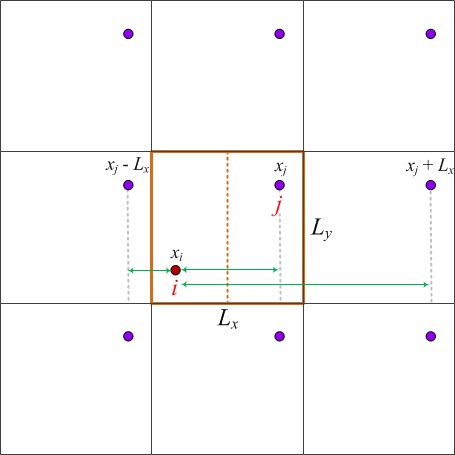
\includegraphics[width=0.6\textwidth]{images/pbc.png}
\caption{Периодические граничные условия (двумерный случай). Фиолетовым цветом показаны образы атома $j$ (образы атома $i$ не приведены)}
\label{fig:pbc}
\end{figure}

\section{Многочастичный потенциал Терсоффа}

\subsection{Вычисление полной энергии}

Согласно \cite{tersoff88} полная энергия $U$ системы (total energy) вычисляется по следующей формуле:
\begin{equation}\label{eq:tersoff88}
U = \displaystyle\sum_{i=1}^{n} U_i = \frac{1}{2}\sum_{i = 1}^{n}\sum_{j = 1 \atop j \neq i}^{n} U_{ij} = \sum_{i = 1}^{n - 1}\sum_{j = i + 1}^{n} U_{ij},
\end{equation}
где $U_{ij}$ -- это энергия связи между атомами $i$ и $j$ (bond energy).
\begin{equation}\label{eq:bondenergy}
U_{ij} = f_C(r_{ij})(a_{ij}f_R(r_{ij}) + b_{ij}f_A(r_{ij})),
\end{equation}
где $r_{ij}$ -- это расстояние между атомами $i$ и $j$, функция $f_R(r_{ij})$ -- это парный потенциал <<отталкивания>> (repulsive pair potential), функция $f_A(r_{ij})$ -- это парный потенциал <<притяжения>> (attractive pair potential), функция $f_C(r_{ij})$ -- это гладкая функция <<отсечки>> (cutoff function).

Зная координаты атомов $\vec{r}_i = (x_i, y_i, z_i)$ и $\vec{r}_j = (x_j, y_j, z_j)$ нетрудно вычислить расстояние между ними
\begin{equation}\label{eq:rij}
r_{ij} = \sqrt{(x_i - x_j)^2 + (y_i - y_j)^2 + (z_i - z_j)^2}.
\end{equation}
\[
f_C(r) =
\begin{cases}
1, &\text{$r < R - D$,}\\
\frac{1}{2} - \frac{1}{2}\sin(\frac{\pi}{2} (r -R) / D), &\text{$R - D < r < R + D$,}\\
0, &\text{$r > R + D$.}
\end{cases}
\]
\begin{equation}
f_R(r) = A \exp (- \lambda_1 r), 
\end{equation}
\begin{equation}
f_A(r) = -B \exp (- \lambda_2 r),
\end{equation}

\begin{equation}
b_{ij} = (1 + \beta^{m_i} \zeta_{ij}^{m_i}) ^ {-\frac{1}{2m_i}}, 
\end{equation}
\begin{equation}
\zeta_{ij} = \displaystyle\sum_{k=1 \atop k \neq i, j}^{n}f_C(r_{ik})g(\Theta_{ijk})\exp(\lambda_{3}^{3}(r_{ij} - r_{ik})^3), 
\end{equation}
\begin{equation}
g(\Theta) = 1 + \frac{c^2}{d^2} - \frac{c^2}{d^2 + (h - \cos\Theta) ^ 2}
\end{equation}

Параметр $\Theta_{ijk}$ -- это угол между связями (векторами) $\vec{r}_{ij}$ и $\vec{r}_{ik}$ (bond angle). Косинус угла $\Theta$ можно найти зная координаты 
векторов $\vec{r}_{ij}$ и  $\vec{r}_{ik}$

\begin{equation}
\vec{r}_{ij} = (x_j - x_i, y_j - y_i, z_j - z_i), 
\end{equation}
\begin{equation}
\vec{r}_{ik} = (x_k - x_i, y_k - y_i, z_k - z_i), 
\end{equation}
\begin{equation}
|\vec{r}_{ij}| = \sqrt{(x_j - x_i)^2 + (y_j - y_i)^2 + (z_j - z_i)^2}, 
\end{equation}
\begin{equation}
|\vec{r}_{ik}| = \sqrt{(x_k - x_i)^2 + (y_k - y_i)^2 + (z_k - z_i)^2}, 
\end{equation}
\begin{equation}
\vec{r}_{ij} \cdot \vec{r}_{ik} = |\vec{r}_{ij}| |\vec{r}_{ik}| \cos\Theta , 
\end{equation}
\begin{equation}
\vec{r}_{ij} \cdot \vec{r}_{ik} = (x_j - x_i)(x_k - x_i) + (y_j - y_i)(y_k - y_i) + (z_j - z_i)(z_k - z_i),
\end{equation}
\begin{equation}
\cos\Theta = \frac{\vec{r}_{ij} \cdot \vec{r}_{ik}} {|\vec{r}_{ij}| |\vec{r}_{ik}|}.
\end{equation}

\begin{equation}
a_{ij} = (1 + \alpha^{m_i} \eta_{ij}^{m_i}) ^ {-\frac{1}{2m_i}},
\end{equation}
\begin{equation}
\eta_{ij} = \displaystyle\sum_{k=1 \atop k \neq i, j}^{n}f_C(r_{ik})\exp(\lambda_{3}^{3}(r_{ij} - r_{ik})^3).
\end{equation}

Параметры $A$, $B$,  $\lambda_1$,  $\lambda_2$,  $\lambda_3$,  $\beta$, $\alpha$, $c$, $d$,  $h$, $m$, $R$, $D$ -- это константы.

\subsection{Вычисление сил}

Обозначим через $\vec{F}_z = (F_{z}^{x}, F_{z}^{y}, F_{z}^{z})$ вектор силы, действующей на атом $z$, а через $\vec{a}_z = (a_{z}^{x}, a_{z}^{y}, a_{z}^{z})$ вектор ускорения атома. 

Тогда уравнение движения (\ref{eq:newtoneq}) атома $z$ можно записать в координатной форме
\begin{equation}
(a_{z}^{x}, a_{z}^{y}, a_{z}^{z}) m_z = (F_{z}^{x}, F_{z}^{y}, F_{z}^{z}).
\end{equation}

Взаимодействие между атомами является потенциальным, по этой причине сила действующая на атом $z$ -- это отрицательный градиент потенциальной энергии системы.
\begin{equation}
\vec{F}_z(\vec{r}_1, \vec{r}_2, \ldots, \vec{r}_n) = - \nabla_z U(\vec{r}_1, \vec{r}_2, \ldots, \vec{r}_n),
\end{equation}
где $\nabla_z$ -- это векторный дифференциальный оператор набла

\begin{equation}
\nabla_z = (\frac{\partial}{\partial x_z}, \frac{\partial}{\partial y_z}, \frac{\partial}{\partial z_z}),
\end{equation}
\begin{equation}
\nabla_z U(\vec{r}_1, \vec{r}_2, \ldots, \vec{r}_n) = (\frac{\partial U}{\partial x_z}, \frac{\partial U}{\partial y_z}, \frac{\partial U}{\partial z_z}).
\end{equation}

Тогда в координатной форме
\begin{equation}
(F_{z}^{x}, F_{z}^{y}, F_{z}^{z}) = - (\frac{\partial U}{\partial x_z}, \frac{\partial U}{\partial y_z}, \frac{\partial U}{\partial z_z}).
\end{equation}
\begin{equation}\label{eq:fx}
F_{z}^{x} = - \frac{\partial U}{\partial x_z} = - \frac{1}{2}\sum_{i = 1}^{n}\sum_{j = 1 \atop j \neq i}^{n} \frac{\partial U_{ij}}{\partial x_z} .
\end{equation}
\begin{equation}\label{eq:fy}
F_{z}^{y} = - \frac{\partial U}{\partial y_z} = - \frac{1}{2}\sum_{i = 1}^{n}\sum_{j = 1 \atop j \neq i}^{n} \frac{\partial U_{ij}}{\partial y_z} .
\end{equation}
\begin{equation}\label{eq:fz}
F_{z}^{z} = - \frac{\partial U}{\partial z_z} = - \frac{1}{2}\sum_{i = 1}^{n}\sum_{j = 1 \atop j \neq i}^{n} \frac{\partial U_{ij}}{\partial z_z} .
\end{equation}

Три выражения (\ref{eq:fx}) -- (\ref{eq:fz}) можно записать в виде одного заменив дифференцирование по координатам $(x_z, y_z, z_z)$ дифференцированием по вектору $\vec{r}_z = (x_z, y_z, z_z)$
\begin{equation}
\vec{F}_z(\vec{r}_1, \vec{r}_2, \ldots, \vec{r}_n)  = - \frac{1}{2}\sum_{i = 1}^{n}\sum_{j = 1 \atop j \neq i}^{n} \frac{\partial U_{ij}}{\partial \vec{r}_z} .
\end{equation}

Найдем градиент функции $U_{ij}$. Для этого необходимо найти производные функции $U_{ij}$ по переменным $x_z$,  $y_z$,  $z_z$.
 \begin{align*}
 \frac{\partial U_{ij}}{\partial x_z} = & \frac{\partial f_C(r_{ij})}{\partial x_z}\left( a_{ij}f_R(r_{ij}) + b_{ij}f_A(r_{ij})\right) + \\
                                                                          & f_C(r_{ij}) \left( \frac{\partial a_{ij}}{\partial x_z}f_R(r_{ij}) + 
                                                                          a_{ij} \frac{\partial f_R(r_{ij})}{\partial x_z} + 
                                                                         \frac{\partial b_{ij}}{\partial x_z}f_A(r_{ij}) + 
                                                                         b_{ij} \frac{\partial f_A(r_{ij})}{\partial x_z} \right),
\end{align*}
 \begin{align*}
 \frac{\partial U_{ij}}{\partial y_z} = & \frac{\partial f_C(r_{ij})}{\partial y_z}\left( a_{ij}f_R(r_{ij}) + b_{ij}f_A(r_{ij})\right) + \\
                                                                          & f_C(r_{ij}) \left( \frac{\partial a_{ij}}{\partial y_z}f_R(r_{ij}) + 
                                                                          a_{ij} \frac{\partial f_R(r_{ij})}{\partial y_z} + 
                                                                         \frac{\partial b_{ij}}{\partial y_z}f_A(r_{ij}) + 
                                                                         b_{ij} \frac{\partial f_A(r_{ij})}{\partial y_z} \right),
\end{align*}
 \begin{align*}
 \frac{\partial U_{ij}}{\partial z_z} = & \frac{\partial f_C(r_{ij})}{\partial z_z}\left( a_{ij}f_R(r_{ij}) + b_{ij}f_A(r_{ij})\right) + \\
                                                                          & f_C(r_{ij}) \left( \frac{\partial a_{ij}}{\partial z_z}f_R(r_{ij}) + 
                                                                          a_{ij} \frac{\partial f_R(r_{ij})}{\partial z_z} + 
                                                                         \frac{\partial b_{ij}}{\partial z_z}f_A(r_{ij}) + 
                                                                         b_{ij} \frac{\partial f_A(r_{ij})}{\partial z_z} \right).
\end{align*} 

Последние три равенства можно записать в компактном виде через производную по вектору $\vec{r}_z$:
\begin{align*}
 \frac{\partial U_{ij}}{\partial \vec{r}_z} = & \frac{\partial f_C(r_{ij})}{\partial \vec{r}_z}\left( a_{ij}f_R(r_{ij}) + b_{ij}f_A(r_{ij})\right) + \\
                                                                          & f_C(r_{ij}) \left( \frac{\partial a_{ij}}{\partial \vec{r}_z}f_R(r_{ij}) + 
                                                                          a_{ij} \frac{\partial f_R(r_{ij})}{\partial \vec{r}_z} + 
                                                                         \frac{\partial b_{ij}}{\partial \vec{r}_z}f_A(r_{ij}) + 
                                                                         b_{ij} \frac{\partial f_A(r_{ij})}{\partial \vec{r}_z} \right).
\end{align*}

Для нахождения производных функции $f_C(r_{ij})$ воспользуемся правилом дифференцирования сложной функции:
\begin{equation}
\frac{\partial f_C(r_{ij})}{\partial x_z} =  \frac{\partial f_C(r_{ij})}{\partial r_{ij}}\frac{\partial r_{ij}}{\partial x_z},
\end{equation}
\begin{equation}
\frac{\partial f_C(r_{ij})}{\partial y_z} =  \frac{\partial f_C(r_{ij})}{\partial r_{ij}}\frac{\partial r_{ij}}{\partial y_z},
\end{equation}
\begin{equation}
\frac{\partial f_C(r_{ij})}{\partial z_z} =  \frac{\partial f_C(r_{ij})}{\partial r_{ij}}\frac{\partial r_{ij}}{\partial z_z},
\end{equation}
\[
\frac{\partial f_C(r_{ij})}{\partial r_{ij}} =
\begin{cases}
0, &\text{$r < R - D$,}\\
- \frac{\pi}{4D}\cos \left(\frac{\pi}{2} (r_{ij} -R) / D\right), &\text{$R - D < r < R + D$,}\\
0, &\text{$r > R + D$,}
\end{cases}
\]
\begin{equation}
r_{ij} = \sqrt{(x_i - x_j)^2 + (y_i - y_j)^2 + (z_i - z_j)^2},
\end{equation}
\[
\frac{\partial r_{ij}}{\partial x_z} =-\frac{1}{2 r_{ij}}\frac{\partial}{\partial x_z}\left(x^2_i - 2 x_i x_j + x^2_j\right) = 
\begin{cases}
\frac{x_i - x_j}{r_{ij}}, &\text{$z = i$,}\\
\frac{x_j - x_i}{r_{ij}}, &\text{$z = j$,}\\
0, &\text{$z \neq i, z \neq j$.}
\end{cases}
\]
\[
\frac{\partial r_{ij}}{\partial y_z} =-\frac{1}{2 r_{ij}}\frac{\partial}{\partial y_z}\left(y^2_i - 2 y_i y_j + y^2_j\right) = 
\begin{cases}
\frac{y_i - y_j}{r_{ij}}, &\text{$z = i$,}\\
\frac{y_j - y_i}{r_{ij}}, &\text{$z = j$,}\\
0, &\text{$z \neq i, z \neq j$.}
\end{cases}
\]
\[
\frac{\partial r_{ij}}{\partial z_z} =-\frac{1}{2 r_{ij}}\frac{\partial}{\partial z_z}\left(z^2_i - 2 z_i z_j + z^2_j\right) = 
\begin{cases}
\frac{z_i - z_j}{r_{ij}}, &\text{$z = i$,}\\
\frac{z_j - z_i}{r_{ij}}, &\text{$z = j$,}\\
0, &\text{$z \neq i, z \neq j$.}
\end{cases}
\]

В компактной форме:
\[
\frac{\partial r_{ij}}{\partial \vec{r}_z} = \frac{\vec {r}_{ij}}{r_{ij}}\left(\delta_{zj} - \delta_{zi}\right) = 
\begin{cases}
-\frac{\vec {r}_{ij}}{r_{ij}}, &\text{$z = i$,}\\
\frac{\vec {r}_{ij}}{r_{ij}}, &\text{$z = j$,}\\
0, &\text{$z \neq i, z \neq j$,}
\end{cases}
\]
где $\delta_{ij}$ -- символ Кронекера
\begin{equation}
\delta_{ij} = \left\{\begin{matrix} 
1, &  i=j,  \\ 
0, &  i \ne j. \end{matrix}\right.
\end{equation}

Окончательно имеем 
\begin{equation}
\frac{\partial f_C(r_{ij})}{\partial \vec{r}_z} =  \frac{\partial f_C(r_{ij})}{\partial r_{ij}} \left[ \frac{\vec {r}_{ij}}{r_{ij}}\left(\delta_{zj} - \delta_{zi}\right)\right].
\end{equation}

Найдем  градиент функции $f_R(r_{ij})$
\begin{equation}
\frac{\partial f_R(r_{ij})}{\partial \vec{r}_z} = \frac{\partial f_R(r_{ij})}{\partial r_{ij}} \frac{\partial r_{ij}}{\partial \vec{r}_z} =  -\lambda_1 A \exp(-\lambda_1  r_{ij}) \left[ \frac{\vec {r}_{ij}}{r_{ij}}\left(\delta_{zj} - \delta_{zi}\right)\right],
\end{equation}

Найдем  градиент функции $f_A(r_{ij})$
\begin{equation}
\frac{\partial f_A(r_{ij})}{\partial \vec{r}_z} = \frac{\partial f_A(r_{ij})}{\partial r_{ij}} \frac{\partial r_{ij}}{\partial \vec{r}_z} =  -\lambda_2 (-B \exp(-\lambda_1  r_{ij})) \left[ \frac{\vec {r}_{ij}}{r_{ij}}\left(\delta_{zj} - \delta_{zi}\right)\right],
\end{equation}

Найдем градиент функции $b_{ij}$
\begin{equation}
\frac{\partial b_{ij}}{\partial \vec{r}_z} = \frac{- \beta^n \zeta^{n-1}_{ij}}{2(1 + \beta^n \zeta^n_{ij})^{\frac{1}{2n} + 1}} \frac{\partial \zeta_{ij}}{\partial \vec{r}_z},
\end{equation}
\begin{align*}
\frac{\partial \zeta_{ij}}{\partial \vec{r}_z} = \displaystyle\sum_{k=1 \atop k \neq i, j}^{n} & \Big( \frac{\partial f_C(r_{ik})}{\partial \vec{r}_z} g(\Theta_{ijk}) \exp(\lambda^3_3(r_{ij} - r_{ik})^3) + \\
                                                                          &    f_C(r_{ik}) \frac{\partial g(\Theta_{ijk})}{\partial \vec{r}_z} \exp(\lambda^3_3(r_{ij} - r_{ik})^3) +\\ 
                                                                          &    f_C(r_{ik}) g(\Theta_{ijk}) \frac{\partial}{\partial \vec{r}_z}\exp(\lambda^3_3(r_{ij} - r_{ik})^3) \Big),
\end{align*}

\begin{equation}
\frac{\partial f_C(r_{ik})}{\partial \vec{r}_z} =  \frac{\partial f_C(r_{ik})}{\partial r_{ik}} \left[ \frac{\vec {r}_{ik}}{r_{ik}}\left(\delta_{zk} - \delta_{zi}\right)\right],
\end{equation}

\begin{equation*}
\frac{\partial}{\partial \vec{r}_z} \exp(\lambda^3_3(r_{ij} - r_{ik})^3) = 3 \lambda^3_3 (r_{ij} - r_{ik})^2 \exp(\lambda^3_3(r_{ij} - r_{ik})^3) 
\left[ \frac{\vec {r}_{ij}}{r_{ij}}(\delta_{zj} - \delta_{zi}) - \frac{\vec {r}_{ik}}{r_{ik}}\left(\delta_{zk} - \delta_{zi}\right)\right],
\end{equation*}

\begin{align*}
\frac{\partial \cos\Theta_{ijk}}{\partial \vec{r}_z}  & =  \frac{\partial}{\partial \vec{r}_z}\left( \vec{r}_{ij}\cdot\vec{r}_{ik}\right) \frac{r_{ij} r_{ik}}{r^2_{ij} r^2_{ik}} -  \frac{(\vec{r}_{ij}\cdot\vec{r}_{ik}) }{r^2_{ij} r^2_{ik}}\frac{\partial}{\partial \vec{r}_z} (r_{ij} r_{ik}) = \\
  & = \frac{\partial}{\partial \vec{r}_z}\left( \vec{r}_{ij}\cdot\vec{r}_{ik}\right) \frac{1}{r_{ij} r_{ik}} -  \cos\Theta_{ijk} \frac{1}{r_{ij} r_{ik}}  \frac{\partial}{\partial \vec{r}_z} (r_{ij} r_{ik}), 
\end{align*}
\[
\frac{\partial}{\partial \vec{r}_z}(\vec{r}_{ij}\cdot\vec{r}_{ik}) = \vec{r}_{ij}(\delta_{zk} - \delta_{zi}) + \vec{r}_{ik}(\delta_{zj} - \delta_{zi}) = 
\begin{cases}
-\vec{r}_{ij} -  \vec{r}_{ik}, &\text{$z = i$,}\\
\vec{r}_{ik}, &\text{$z = j$,}\\
\vec{r}_{ij}, &\text{$z = k$,}\\
0, &\text{$z \neq i, j, k$,}
\end{cases}
\]
\begin{align*}
\frac{\partial}{\partial \vec{r}_z}(r_{ij}r_{ik})  & = \frac{\partial r_{ij}}{\partial \vec{r}_z}r_{ik} +  r_{ij} \frac{\partial r_{ik}}{\partial \vec{r}_z} = \\
& = \frac{\vec {r}_{ij}}{r_{ij}}(\delta_{zj} - \delta_{zi})r_{ik} + r_{ij}\frac{\vec {r}_{ik}}{r_{ik}}\left(\delta_{zk} - \delta_{zi}\right)
\end{align*}

Учитывая последние два равенства получаем
\begin{align*}
\frac{\partial \cos\Theta_{ijk}}{\partial \vec{r}_z}  & =  \frac{\vec{r}_{ij}(\delta_{zk} - \delta_{zi}) + \vec{r}_{ik}(\delta_{zj} - \delta_{zi})}{r_{ij}r_{ik}} -
\cos\Theta_{ijk} \left[ \frac{\vec {r}_{ij}}{r^2_{ij}}(\delta_{zj} - \delta_{zi}) + \frac{\vec {r}_{ik}}{r^2_{ik}}\left(\delta_{zk} - \delta_{zi}\right) \right]. 
\end{align*}

Найдем градиент функции $a_{ij}$
\begin{equation}
\frac{\partial a_{ij}}{\partial \vec{r}_z} = \frac{- \alpha^n \eta^{n-1}_{ij}}{2(1 + \alpha^n \eta^n_{ij})^{\frac{1}{2n} + 1}} \frac{\partial \eta_{ij}}{\partial \vec{r}_z},
\end{equation}
\begin{equation*}
\frac{\partial \eta_{ij}}{\partial \vec{r}_z} = \displaystyle\sum_{k=1 \atop k \neq i, j}^{n} \Big( \frac{\partial f_C(r_{ik})}{\partial \vec{r}_z}  \exp(\lambda^3_3(r_{ij} - r_{ik})^3) +  f_C(r_{ik}) \frac{\partial}{\partial \vec{r}_z}\exp(\lambda^3_3(r_{ij} - r_{ik})^3) \Big).
\end{equation*}

\section{Многочастичный потенциал Терсоффа 2}

\subsection{Вычисление полной энергии (Терсофф 2)}

Согласно \cite{tersoff89} полная энергия $U$ системы (total energy) вычисляется по следующей формуле:
\begin{equation}\label{eq:tersoff89}
U = \displaystyle\sum_{i=1}^{n} U_i = \frac{1}{2}\sum_{i = 1}^{n}\sum_{j = 1 \atop j \neq i}^{n} U_{ij} = \sum_{i = 1}^{n - 1}\sum_{j = i + 1}^{n} U_{ij},
\end{equation}
где $U_{ij}$ -- это энергия связи между атомами $i$ и $j$ (bond energy).
\begin{equation}\label{eq:tersoff89_bondenergy}
U_{ij} = f_C(r_{ij})(f_R(r_{ij}) + b_{ij}f_A(r_{ij})),
\end{equation}
где $r_{ij}$ -- это расстояние между атомами $i$ и $j$, функция $f_R(r_{ij})$ -- это парный потенциал <<отталкивания>> (repulsive pair potential), функция $f_A(r_{ij})$ -- это парный потенциал <<притяжения>> (attractive pair potential), функция $f_C(r_{ij})$ -- это гладкая функция <<отсечки>> (cutoff function).

Зная координаты атомов $\vec{r}_i = (x_i, y_i, z_i)$ и $\vec{r}_j = (x_j, y_j, z_j)$ нетрудно вычислить расстояние между ними
\begin{equation}\label{eq:tersoff89_rij}
r_{ij} = \sqrt{(x_i - x_j)^2 + (y_i - y_j)^2 + (z_i - z_j)^2}.
\end{equation}
\[
f_C(r) =
\begin{cases}
	1, &\text{$r_{ij} < R_{ij}$,}\\
	\frac{1}{2} - \frac{1}{2}\cos(\pi (r_{ij} - R_{ij}) / (S_{ij} - R_{ij})), &\text{$R_{ij}< r_{ij} < S_{ij}$,}\\
	0, &\text{$r_{ij} > S_{ij}$.}
\end{cases}
\]
\begin{equation}
f_R(r_{ij}) = A_{ij} \exp (- \lambda_{ij} r_{ij}), 
\end{equation}
\begin{equation}
f_A(r_{ij}) = -B_{ij} \exp (- \lambda_{ij} r_{ij}),
\end{equation}

\begin{equation}
b_{ij} = \chi_{ij} 	(1 + \beta_{i}^{m_i} \zeta_{ij}^{m_i}) ^ {-\frac{1}{2m_i}}, 
\end{equation}
\begin{equation}
\zeta_{ij} = \displaystyle\sum_{k=1 \atop k \neq i, j}^{n}f_C(r_{ik})\omega_{ik}g(\Theta_{ijk}), 
\end{equation}
\begin{equation}
g(\Theta_{ijk}) = 1 + \frac{c_i^2}{d_i^2} - \frac{c_i^2}{d_i^2 + (h_i - \cos\Theta_{ijk}) ^ 2}
\end{equation}
\begin{equation}
\lambda_{ij} = (\lambda_i + \lambda_j) / 2
\end{equation}
\begin{equation}
\mu_{ij} = (\mu_i + \mu_j) / 2
\end{equation}
\begin{equation}
A_{ij} = \sqrt{A_i A_j}
\end{equation}
\begin{equation}
B_{ij} = \sqrt{B_i B_j}
\end{equation}
\begin{equation}
R_{ij} = \sqrt{R_i R_j}
\end{equation}
\begin{equation}
S_{ij} = \sqrt{S_i S_j}
\end{equation}

Параметр $\Theta_{ijk}$ -- это угол между связями (векторами) $\vec{r}_{ij}$ и $\vec{r}_{ik}$ (bond angle). Косинус угла $\Theta$ можно найти зная координаты 
векторов $\vec{r}_{ij}$ и  $\vec{r}_{ik}$

\begin{equation}
\vec{r}_{ij} = (x_j - x_i, y_j - y_i, z_j - z_i), 
\end{equation}
\begin{equation}
\vec{r}_{ik} = (x_k - x_i, y_k - y_i, z_k - z_i), 
\end{equation}
\begin{equation}
|\vec{r}_{ij}| = \sqrt{(x_j - x_i)^2 + (y_j - y_i)^2 + (z_j - z_i)^2}, 
\end{equation}
\begin{equation}
|\vec{r}_{ik}| = \sqrt{(x_k - x_i)^2 + (y_k - y_i)^2 + (z_k - z_i)^2}, 
\end{equation}
\begin{equation}
\vec{r}_{ij} \cdot \vec{r}_{ik} = |\vec{r}_{ij}| |\vec{r}_{ik}| \cos\Theta , 
\end{equation}
\begin{equation}
\vec{r}_{ij} \cdot \vec{r}_{ik} = (x_j - x_i)(x_k - x_i) + (y_j - y_i)(y_k - y_i) + (z_j - z_i)(z_k - z_i),
\end{equation}
\begin{equation}
\cos\Theta = \frac{\vec{r}_{ij} \cdot \vec{r}_{ik}} {|\vec{r}_{ij}| |\vec{r}_{ik}|}.
\end{equation}

Параметры $A_{ij}$, $B_{ij}$, $R_{ij}$, $S_{ij}$, $\lambda_{ij}$, $\mu_{ij}$, $c_i$, $d_i$, $h_i$, $m_i$ -- это константы.

\subsection{Вычисление сил (Терсофф 2)}

Обозначим через $\vec{F}_z = (F_{z}^{x}, F_{z}^{y}, F_{z}^{z})$ вектор силы, действующей на атом $z$, а через $\vec{a}_z = (a_{z}^{x}, a_{z}^{y}, a_{z}^{z})$ вектор ускорения атома. 

Тогда уравнение движения (\ref{eq:newtoneq}) атома $z$ можно записать в координатной форме
\begin{equation}
(a_{z}^{x}, a_{z}^{y}, a_{z}^{z}) m_z = (F_{z}^{x}, F_{z}^{y}, F_{z}^{z}).
\end{equation}

Взаимодействие между атомами является потенциальным, по этой причине сила действующая на атом $z$ -- это отрицательный градиент потенциальной энергии системы.
\begin{equation}
\vec{F}_z(\vec{r}_1, \vec{r}_2, \ldots, \vec{r}_n) = - \nabla_z U(\vec{r}_1, \vec{r}_2, \ldots, \vec{r}_n),
\end{equation}
где $\nabla_z$ -- это векторный дифференциальный оператор набла

\begin{equation}
\nabla_z = (\frac{\partial}{\partial x_z}, \frac{\partial}{\partial y_z}, \frac{\partial}{\partial z_z}),
\end{equation}
\begin{equation}
\nabla_z U(\vec{r}_1, \vec{r}_2, \ldots, \vec{r}_n) = (\frac{\partial U}{\partial x_z}, \frac{\partial U}{\partial y_z}, \frac{\partial U}{\partial z_z}).
\end{equation}

Тогда в координатной форме
\begin{equation}
(F_{z}^{x}, F_{z}^{y}, F_{z}^{z}) = - (\frac{\partial U}{\partial x_z}, \frac{\partial U}{\partial y_z}, \frac{\partial U}{\partial z_z}).
\end{equation}
\begin{equation}\label{eq:tersoff2_fx}
F_{z}^{x} = - \frac{\partial U}{\partial x_z} = - \frac{1}{2}\sum_{i = 1}^{n}\sum_{j = 1 \atop j \neq i}^{n} \frac{\partial U_{ij}}{\partial x_z} .
\end{equation}
\begin{equation}\label{eq:tersoff2_fy}
F_{z}^{y} = - \frac{\partial U}{\partial y_z} = - \frac{1}{2}\sum_{i = 1}^{n}\sum_{j = 1 \atop j \neq i}^{n} \frac{\partial U_{ij}}{\partial y_z} .
\end{equation}
\begin{equation}\label{eq:tersoff2_fz}
F_{z}^{z} = - \frac{\partial U}{\partial z_z} = - \frac{1}{2}\sum_{i = 1}^{n}\sum_{j = 1 \atop j \neq i}^{n} \frac{\partial U_{ij}}{\partial z_z} .
\end{equation}

Три выражения (\ref{eq:tersoff2_fx}) -- (\ref{eq:tersoff2_fz}) можно записать в виде одного заменив дифференцирование по координатам $(x_z, y_z, z_z)$ дифференцированием по вектору $\vec{r}_z = (x_z, y_z, z_z)$
\begin{equation}
\vec{F}_z(\vec{r}_1, \vec{r}_2, \ldots, \vec{r}_n)  = - \frac{1}{2}\sum_{i = 1}^{n}\sum_{j = 1 \atop j \neq i}^{n} \frac{\partial U_{ij}}{\partial \vec{r}_z} .
\end{equation}

Найдем градиент функции $U_{ij}$. Для этого необходимо найти производные функции $U_{ij}$ по переменным $x_z$,  $y_z$,  $z_z$.

\begin{align*}
 \frac{\partial U_{ij}}{\partial x_z} = & \frac{\partial f_C(r_{ij})}{\partial x_z}\left( f_R(r_{ij}) + b_{ij}f_A(r_{ij})\right) + \\
	& f_C(r_{ij}) \left( \frac{\partial f_R(r_{ij})}{\partial x_z} + 
	\frac{\partial b_{ij}}{\partial x_z}f_A(r_{ij}) +
	b_{ij} \frac{\partial f_A(r_{ij})}{\partial x_z} \right),
\end{align*}

\begin{align*}
 \frac{\partial U_{ij}}{\partial y_z} = & \frac{\partial f_C(r_{ij})}{\partial y_z}\left( f_R(r_{ij}) + b_{ij}f_A(r_{ij})\right) + \\
	& f_C(r_{ij}) \left( \frac{\partial f_R(r_{ij})}{\partial y_z} + 
	\frac{\partial b_{ij}}{\partial y_z}f_A(r_{ij}) +
	b_{ij} \frac{\partial f_A(r_{ij})}{\partial y_z} \right),
\end{align*}

\begin{align*}
 \frac{\partial U_{ij}}{\partial z_z} = & \frac{\partial f_C(r_{ij})}{\partial z_z}\left( f_R(r_{ij}) + b_{ij}f_A(r_{ij})\right) + \\
	& f_C(r_{ij}) \left( \frac{\partial f_R(r_{ij})}{\partial z_z} + 
	\frac{\partial b_{ij}}{\partial z_z}f_A(r_{ij}) +
	b_{ij} \frac{\partial f_A(r_{ij})}{\partial z_z} \right),
\end{align*}

Последние три равенства можно записать в компактном виде через производную по вектору $\vec{r}_z$:
\begin{align*}
 \frac{\partial U_{ij}}{\partial \vec{r}_z} = & \frac{\partial f_C(r_{ij})}{\partial \vec{r}_z}\left( f_R(r_{ij}) + b_{ij}f_A(r_{ij})\right) + \\
	& f_C(r_{ij}) \left( \frac{\partial f_R(r_{ij})}																									{\partial \vec{r}_z} + 
	\frac{\partial b_{ij}}{\partial \vec{r}_z}f_A(r_{ij}) +
	b_{ij} \frac{\partial f_A(r_{ij})}{\partial \vec{r}_z} \right),
\end{align*}

Для нахождения производных функции $f_C(r_{ij})$ воспользуемся правилом дифференцирования сложной функции:
\begin{equation}
\frac{\partial f_C(r_{ij})}{\partial x_z} =  \frac{\partial f_C(r_{ij})}{\partial r_{ij}}\frac{\partial r_{ij}}{\partial x_z},
\end{equation}
\begin{equation}
\frac{\partial f_C(r_{ij})}{\partial y_z} =  \frac{\partial f_C(r_{ij})}{\partial r_{ij}}\frac{\partial r_{ij}}{\partial y_z},
\end{equation}
\begin{equation}
\frac{\partial f_C(r_{ij})}{\partial z_z} =  \frac{\partial f_C(r_{ij})}{\partial r_{ij}}\frac{\partial r_{ij}}{\partial z_z},
\end{equation}

\[
\frac{\partial f_C(r_{ij})}{\partial r_{ij}} =
\begin{cases}
0, &\text{$r_{ij} < R_{ij}$,}\\
- \frac{\pi}{2(S_{ij} - R_{ij})}\cos \left(\pi (r_{ij} - R_{ij}) / (S_{ij} - R_{ij})\right), &\text{$R_{ij}< r_{ij} < S_{ij}$,}\\
0, &\text{$r_{ij} > S_{ij}$,}
\end{cases}
\]
\begin{equation}
r_{ij} = \sqrt{(x_i - x_j)^2 + (y_i - y_j)^2 + (z_i - z_j)^2},
\end{equation}
\[
\frac{\partial r_{ij}}{\partial x_z} =-\frac{1}{2 r_{ij}}\frac{\partial}{\partial x_z}\left(x^2_i - 2 x_i x_j + x^2_j\right) = 
\begin{cases}
\frac{x_i - x_j}{r_{ij}}, &\text{$z = i$,}\\
\frac{x_j - x_i}{r_{ij}}, &\text{$z = j$,}\\
0, &\text{$z \neq i, z \neq j$.}
\end{cases}
\]
\[
\frac{\partial r_{ij}}{\partial y_z} =-\frac{1}{2 r_{ij}}\frac{\partial}{\partial y_z}\left(y^2_i - 2 y_i y_j + y^2_j\right) = 
\begin{cases}
\frac{y_i - y_j}{r_{ij}}, &\text{$z = i$,}\\
\frac{y_j - y_i}{r_{ij}}, &\text{$z = j$,}\\
0, &\text{$z \neq i, z \neq j$.}
\end{cases}
\]
\[
\frac{\partial r_{ij}}{\partial z_z} =-\frac{1}{2 r_{ij}}\frac{\partial}{\partial z_z}\left(z^2_i - 2 z_i z_j + z^2_j\right) = 
\begin{cases}
\frac{z_i - z_j}{r_{ij}}, &\text{$z = i$,}\\
\frac{z_j - z_i}{r_{ij}}, &\text{$z = j$,}\\
0, &\text{$z \neq i, z \neq j$.}
\end{cases}
\]

В компактной форме:
\[
\frac{\partial r_{ij}}{\partial \vec{r}_z} = \frac{\vec {r}_{ij}}{r_{ij}}\left(\delta_{zj} - \delta_{zi}\right) = 
\begin{cases}
-\frac{\vec {r}_{ij}}{r_{ij}}, &\text{$z = i$,}\\
\frac{\vec {r}_{ij}}{r_{ij}}, &\text{$z = j$,}\\
0, &\text{$z \neq i, z \neq j$,}
\end{cases}
\]
где $\delta_{ij}$ -- символ Кронекера
\begin{equation}
\delta_{ij} = \left\{\begin{matrix} 
1, &  i=j,  \\ 
0, &  i \ne j. \end{matrix}\right.
\end{equation}

Окончательно имеем 
\begin{equation}
\frac{\partial f_C(r_{ij})}{\partial \vec{r}_z} =  \frac{\partial f_C(r_{ij})}{\partial r_{ij}} \left[ \frac{\vec {r}_{ij}}{r_{ij}}\left(\delta_{zj} - \delta_{zi}\right)\right].
\end{equation}

Найдем  градиент функции $f_R(r_{ij})$
\begin{equation}
\frac{\partial f_R(r_{ij})}{\partial \vec{r}_z} = \frac{\partial f_R(r_{ij})}{\partial r_{ij}} \frac{\partial r_{ij}}{\partial \vec{r}_z} =  -\lambda_{ij} A_{ij} \exp(-\lambda_{ij}  r_{ij}) \left[ \frac{\vec {r}_{ij}}{r_{ij}}\left(\delta_{zj} - \delta_{zi}\right)\right],
\end{equation}

Найдем  градиент функции $f_A(r_{ij})$
\begin{equation}
\frac{\partial f_A(r_{ij})}{\partial \vec{r}_z} = \frac{\partial f_A(r_{ij})}{\partial r_{ij}} \frac{\partial r_{ij}}{\partial \vec{r}_z} =  -\lambda_{ij} (-B_{ij} \exp(-\lambda_{ij} r_{ij})) \left[ \frac{\vec {r}_{ij}}{r_{ij}}\left(\delta_{zj} - \delta_{zi}\right)\right],
\end{equation}

Найдем градиент функции $b_{ij}$
\begin{equation}
\frac{\partial b_{ij}}{\partial \vec{r}_z} = \chi_{ij} \frac{- \beta_i^{m_i} \zeta^{{m_i}-1}_{ij}}{2(1 + \beta_i^{m_i} \zeta^{m_i}_{ij})^{\frac{1}{2m_i} + 1}} \frac{\partial \zeta_{ij}}{\partial \vec{r}_z},
\end{equation}

\begin{align*}
\frac{\partial \zeta_{ij}}{\partial \vec{r}_z} = \displaystyle\sum_{k=1 \atop k \neq i, j}^{n} & \Big( \frac{\partial f_C(r_{ik})}{\partial \vec{r}_z} \omega_{ik} g(\Theta_{ijk}) + 
f_C(r_{ik}) \omega_{ik} \frac{\partial g(\Theta_{ijk})}{\partial \vec{r}_z} \Big),
\end{align*}

\begin{equation}
\frac{\partial f_C(r_{ik})}{\partial \vec{r}_z} =  \frac{\partial f_C(r_{ik})}{\partial r_{ik}} \left[ \frac{\vec {r}_{ik}}{r_{ik}}\left(\delta_{zk} - \delta_{zi}\right)\right],
\end{equation}

Найдем градиент функции $g(\Theta_{ijk})$

\begin{equation}
\frac{\partial g(\Theta_{ijk})}{\partial \vec{r}_z} = 
	-\frac{2c_i^2 (h_i - \cos\Theta_{ijk})}{(d_i^2 + (h_i - \cos\Theta_{ijk})^2)^2} \cdot
	\frac{\partial \cos\Theta_{ijk}}{\partial \vec{r}_z}
\end{equation}

\begin{align*}
\frac{\partial \cos\Theta_{ijk}}{\partial \vec{r}_z} & =  \frac{\partial}{\partial \vec{r}_z}\left( \vec{r}_{ij}\cdot\vec{r}_{ik}\right) \frac{r_{ij} r_{ik}}{r^2_{ij} r^2_{ik}} -  \frac{(\vec{r}_{ij}\cdot\vec{r}_{ik}) }{r^2_{ij} r^2_{ik}}\frac{\partial}{\partial \vec{r}_z} (r_{ij} r_{ik}) = \\
  & = \frac{\partial}{\partial \vec{r}_z}\left( \vec{r}_{ij}\cdot\vec{r}_{ik}\right) \frac{1}{r_{ij} r_{ik}} -  \cos\Theta_{ijk} \frac{1}{r_{ij} r_{ik}}  \frac{\partial}{\partial \vec{r}_z} (r_{ij} r_{ik}), 
\end{align*}
\[
\frac{\partial}{\partial \vec{r}_z}(\vec{r}_{ij}\cdot\vec{r}_{ik}) = \vec{r}_{ij}(\delta_{zk} - \delta_{zi}) + \vec{r}_{ik}(\delta_{zj} - \delta_{zi}) = 
\begin{cases}
-\vec{r}_{ij} -  \vec{r}_{ik}, &\text{$z = i$,}\\
\vec{r}_{ik}, &\text{$z = j$,}\\
\vec{r}_{ij}, &\text{$z = k$,}\\
0, &\text{$z \neq i, j, k$,}
\end{cases}
\]
\begin{align*}
\frac{\partial}{\partial \vec{r}_z}(r_{ij}r_{ik})  & = \frac{\partial r_{ij}}{\partial \vec{r}_z}r_{ik} +  r_{ij} \frac{\partial r_{ik}}{\partial \vec{r}_z} = \\
& = \frac{\vec {r}_{ij}}{r_{ij}}(\delta_{zj} - \delta_{zi})r_{ik} + r_{ij}\frac{\vec {r}_{ik}}{r_{ik}}\left(\delta_{zk} - \delta_{zi}\right)
\end{align*}

Учитывая последние два равенства получаем
\begin{align*}
\frac{\partial \cos\Theta_{ijk}}{\partial \vec{r}_z}  & =  \frac{\vec{r}_{ij}(\delta_{zk} - \delta_{zi}) + \vec{r}_{ik}(\delta_{zj} - \delta_{zi})}{r_{ij}r_{ik}} -
\cos\Theta_{ijk} \left[ \frac{\vec {r}_{ij}}{r^2_{ij}}(\delta_{zj} - \delta_{zi}) + \frac{\vec {r}_{ik}}{r^2_{ik}}\left(\delta_{zk} - \delta_{zi}\right) \right]. 
\end{align*}

\section{Оптимизация вычислений взаимодействий между атомами}

\subsection{Метод ячеек}

Разобъем область моделирования (и ее образы) на ячейки (cells) размера 

   
Мы рассматриваем характеристики системы атомов при постоянной плотности. Частицы находятся внутри ячейки (параллелепипеда) размера $L_x \times L_y \times L_z$. 

Грани ячейки порождают нежелательные поверхности, от которых атомы отражаются и возвращаются в ячейку.  Таким образом грани вносят значительный вклад в любую характеристику системы.

Для уменьшения влияния гранией введем \textit{периодические граничные условия} (periodic boundary conditions -- PBC) -- базовая ячейка повторяется (тиражируется) бесконечное число раз во всех направлениях. Таким образом, любой атом c координатой $\vec{r}_i$ имеет бесконечное количество своих образов (images) с координатами 


\section{Структура алгоритма}

\begin{enumerate}
\item Инициализируем среду моделирования (параметры атомов, simulation box).
\item Загружаем/генерируем начальные положения атомов $\vec{r}_i(0)$, их скорости $\vec{v}_i(0)$
\item Формируем локальную окрестность каждого атома (verlet list, linked cell)
\item Вычисляем силы $\vec{F}_i(0)$ и по ним начальные ускорения атомов $\vec{a}_i(0)$
\item Выполняем шаги по времени $t = \Delta t, 2\Delta t, \ldots, N\Delta t$
    \begin{enumerate}
    \item Первый шаг алгоритма Velocity Verlet\\
    $\vec{v}_i(t + \frac{1}{2}\Delta t) = \vec{v}_i(t) +  \frac{1}{2}\vec{a}_i(t) \Delta t$\\
    $\vec{r}_i(t + \Delta t) = \vec{r}_i(t) +  \vec{v}_i(t + \frac{1}{2}\Delta t) \Delta t$ 
    \item Вычисляем силы и по ним ускорения атомов \\$\vec{a}_i(t + \Delta t) = \frac{1}{m} \vec{F}_i(\vec{r}_1(t + \Delta t), \vec{r}_2(t + \Delta t), \ldots, \vec{r}_n(t + \Delta t))$
    \item Вычисляем скорость атомов \\$\vec{v}_i(t + \Delta t) = \vec{v}_i(t + \frac{1}{2}\Delta t) +  \frac{1}{2}  \vec{a}_i(t + \Delta t) \Delta t$
    \end{enumerate}
 
\end{enumerate}

TODO: локальная окрестность каждого атома, PBC

\section{Обзор предшествующих работ}

Основные пакеты: Andersen (Tersoff\_2), LAMMPS (Tersoff\_1, Tersoff\_2), CP2K, MBN Explorer.


\bibliographystyle{unsrt}
\bibliography{md-intro}

\end{document}